\documentclass[12pt,a4paper]{article}
\usepackage[utf8]{inputenc}
\usepackage[english]{babel}
\usepackage{amsmath}
\usepackage{amsfonts}
\usepackage{amssymb}
\usepackage{graphicx}
\usepackage[left=2cm,right=2cm,top=2cm,bottom=2cm]{geometry}
\author{Baptiste Rouger}
\title{Statistics : Final Exam}
\begin{document}
\maketitle

If nothing is mentioned, I will use a 5\% confidence interval.
\section*{Exercise 1}
\subsection*{Question 1}
The population is the cones in the eye. The variable is the number of the L type of cone. In this case, the sample is the N cones observed.

\subsection*{Question 2}
The population is the humans, the variable is the percentage of cone, and the sample here is the 10 people we observe.\\

The correlation test show, for $M_\%$ and $L_\%$ (\textsc{Figure}~\ref{corr1}), a correlation coefficient of $-0.96$ with a p-value of $1.0620\cdot 10^{-5}$. As the correlation coefficient is near from $-1$ and the p-value far under $0.05$, this shows that there is actually a correlation between $M_\%$ and $L_\%$, as the p-value is far lower than 0.05.\\

For $M_\% - L_\%$ and $S_\%$ (\textsc{Figure}~\ref{corr2}), the correlation coefficient is $0.192$ and the p-value $0.5951$. As the correlation coefficient is near to $0$ and the p-value is far above $0.05$, this test does not show a correlation between $M_\% - L_\%$ and $S_\%$ for this sample.\\

We can be pretty confident in the first correlation test, as the p-value is really low. Though, for the second test, it seems pretty unlikely that there actually is a correlation, as the correlation coefficient is far from 1 and the p-value far above 0.05. This sample could be repeated to check this.

\begin{figure}
  \begin{center}
    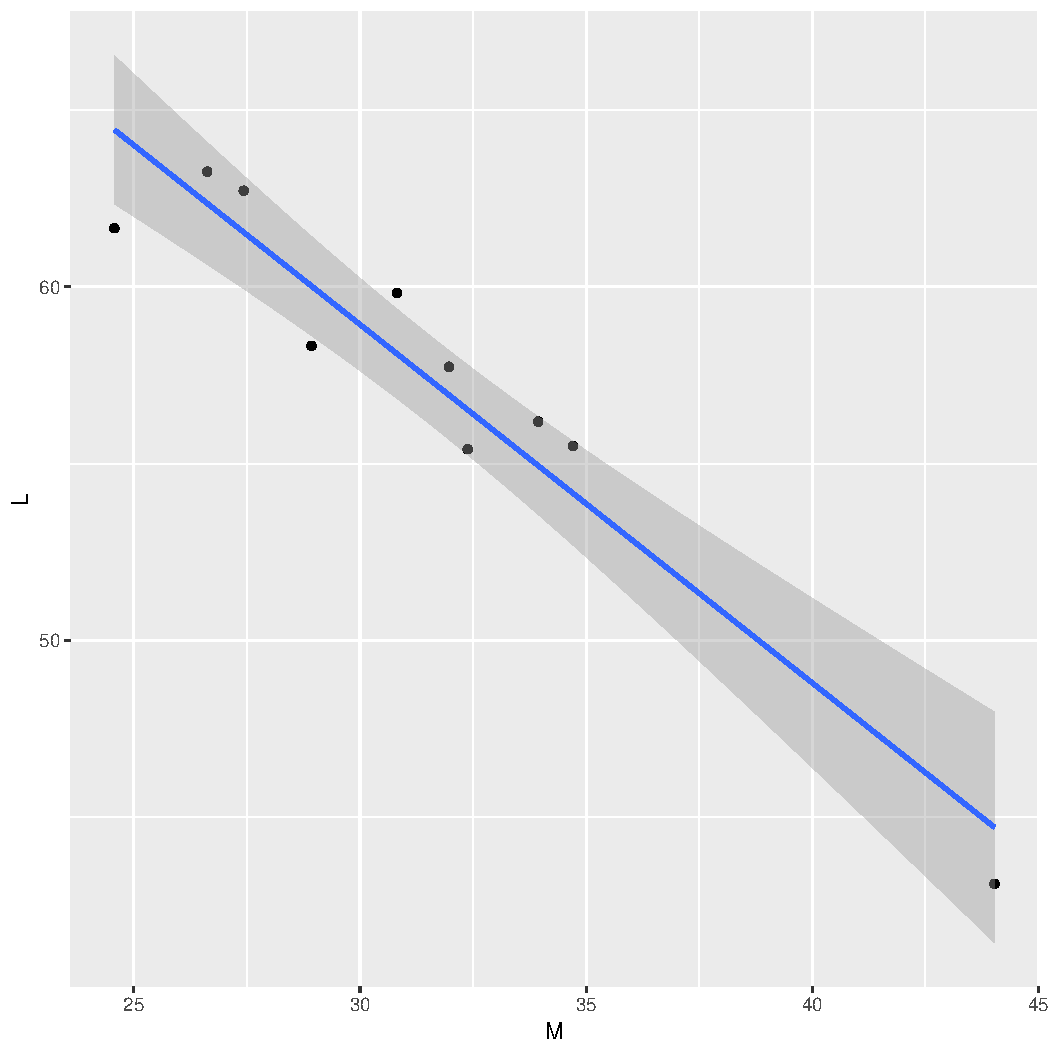
\includegraphics[width=0.6\linewidth]{corr1.pdf}
    \caption{Plot of $M_\%$ against $L_\%$}
    \label{corr1}
  \end{center}
\end{figure}

\begin{figure}
  \begin{center}
    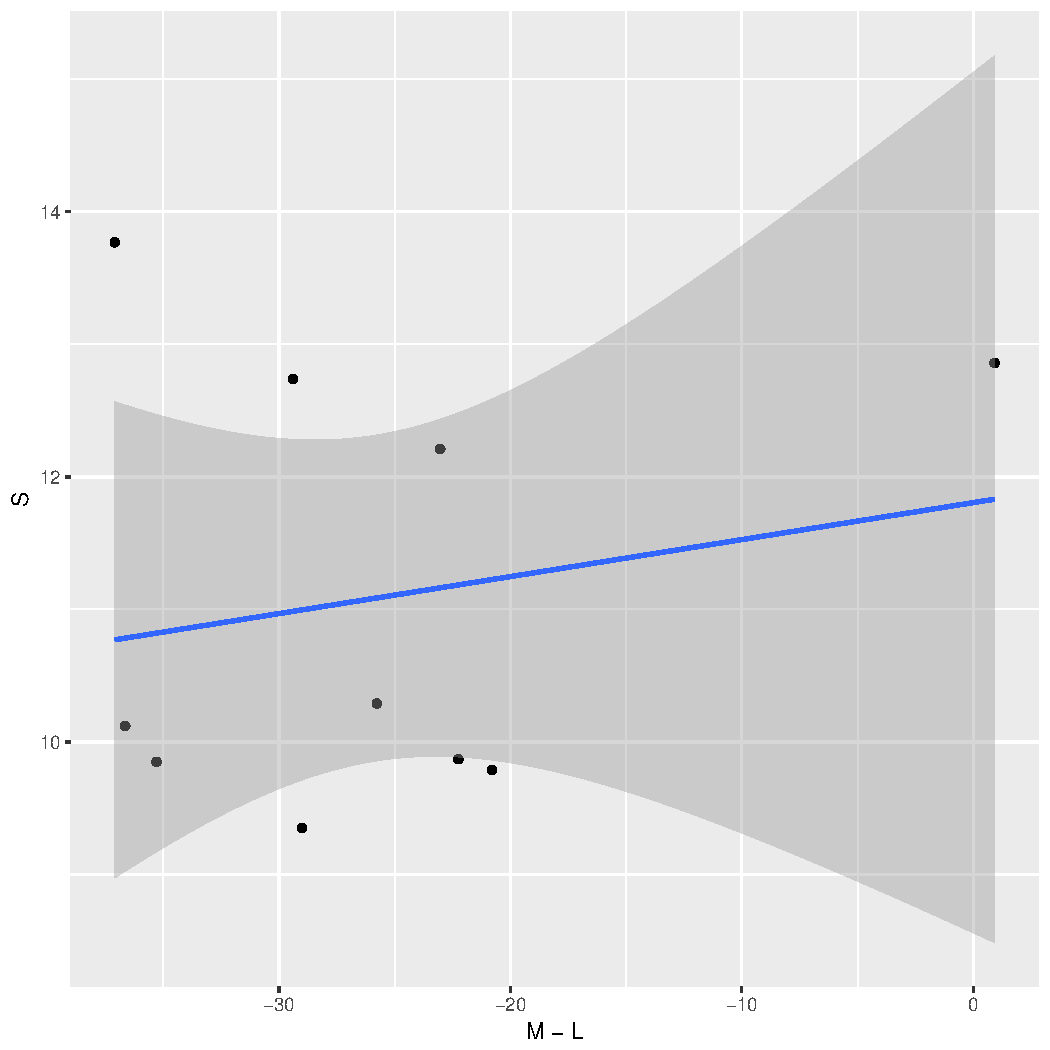
\includegraphics[width=0.6\linewidth]{corr2.pdf}
    \caption{Plot of $M_\% - L_\%$ against $S_\%$}
    \label{corr2}
  \end{center}
\end{figure}

\newpage
\section*{Exercise 2}
\subsection*{Question 1}
Here, we want to see if one of the sample is not equal to the other (i.e the brand put less powder than the other). Thus, our null hypothesis $H_0$ will be :\\
\begin{center}$H_0$ : the two brands tuned the machine to put the same weight of powder.\end{center}

We then perform a two sample Student analysis with R to see if the two means are equal, and we get a p-value of $0.03481$. We can see here that we refute the null hypothesis. Thus, we can say that the brand A and B tuned the machine in differrent ways.\\

We perform an other two sample Student analysis with the null hypothesis being \begin{center}$H_0$ : the brand A put more powder than B.\end{center}
We then get a p-value from the t-test of $0.0174$, which means that we reject the null hypothesis. Thus, A puts significantly less powder than B.

\subsection*{Question 2}
We want to check if the two brands actually sell 100mg of powder. For both brands, our null hypothesis will then be :\\
$H_0$ : the brand sell doses of 100mg.\\
We perform a one sample Student analysis for both brand samples. We get for the brand A a p-value of $0.06565$. This shows us that we can not refute the null hypothesis, and thus we cannot tell that the brand A sells, in mean, less or more than 100mg of powder.\\
For the brand B, after performing the same test, we get a p-value of $0.0001213$. This p-value is far under $0.05$, thus we refute the null hypothesis and can say that the brand B do not sell, in mean, 100mg of powder.\\

I then wanted to know if B was selling more or less than 100mg, as they do not sell exactly this weight. I used a one sample T-test with $H_0$ being $\mu_B > 100mg$. I got a p-value of $0.9999$, meaning that we do not reject the null hypothesis. We can then determine that B is not actually cheating because it sells, in mean, more than 100mg of powder.

\section*{Exercise 3}
\subsection*{Question 1}
Using visual inspection first (\textsc{Figure}~\ref{corr3}), we observe a pretty good correlation between the two barometers. As we can see in \textsc{Figure}, all the points are around a line (here the linear model regression in blue, with confidence interval of 95\%).\\

\begin{figure}
  \begin{center}
    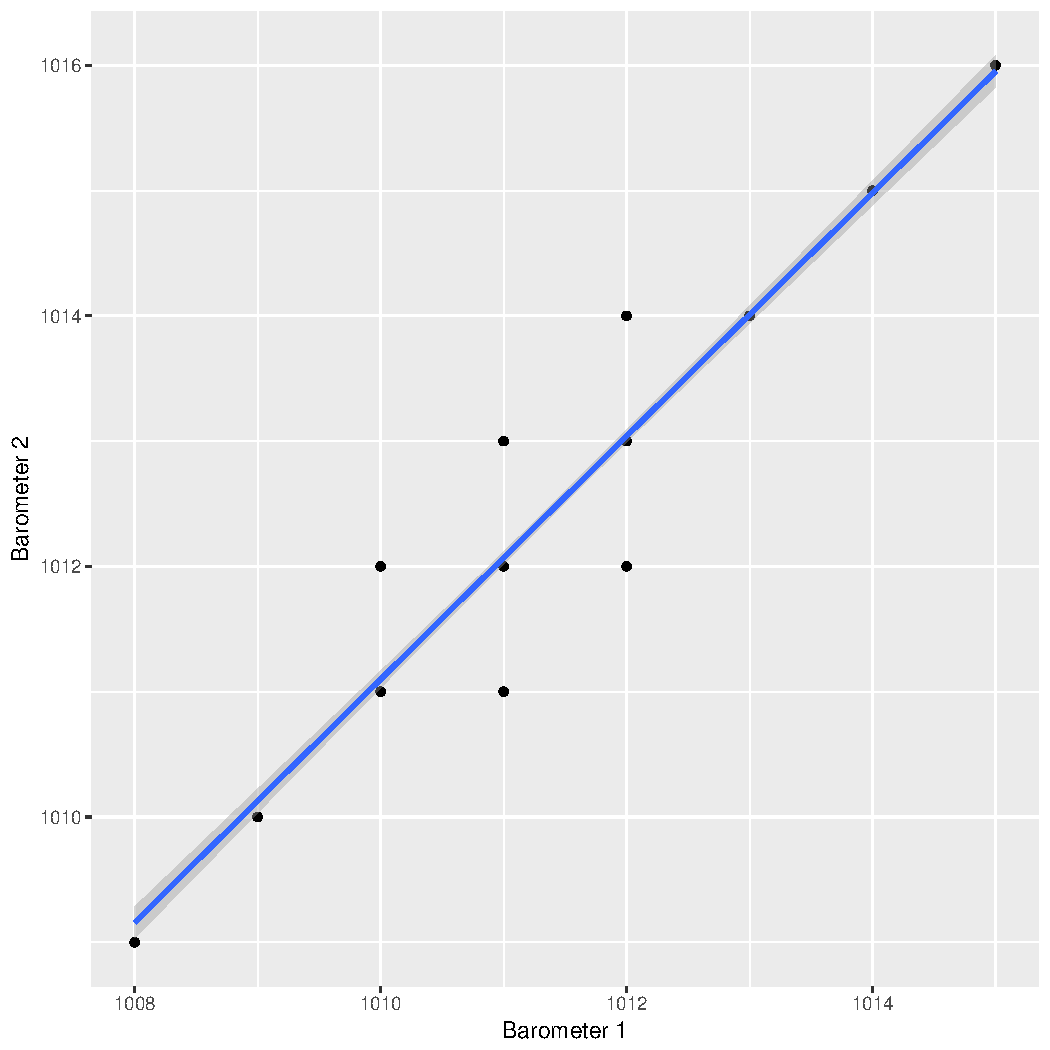
\includegraphics[width=0.6\linewidth]{corr3.pdf}
    \caption{Plot of the data of the second barometer against the first one}
    \label{corr3}
  \end{center}
\end{figure}

We then use the correlation function of R to see if this correlation exists (with the Spearman option). We obtain a correlation coefficient of $0.96$ wich is close to 1, and a p-value of 0 (it is likely that the actual value is higher, but it is the value returned in the matrix by R. It seems this value is under $1\cdot 10^{-5}$.). We can conclude that there is a significant correlation between the two barometers.

\subsection*{Question 2}
Using the built-in lm R function, we find a equation of the linear model such as $y = 0.97035x + 31.04732$. We then use the summary function on the linear model, and see that the signification level is $<2.2 \cdot 10^{-16}$. Thus, we can say that our linear model is significant.

\subsection*{Question 3}
Using the built-in R function for the Kolmogorov-Smirnov test, I try the hypothesis $H_0$ : The two samples have the same distribution.\\
I get the result such as $D = 0.60174$ and a p-value such as $2.2e-16$. As D is lower than $1.96$ which corresponds to the $5\%$ confidence interval and the p-value far under $0.05$; we can say that the two samples are the statistically the same.\\

\subsection*{Question 4}
Please find the data presentation in the \textsc{Figure}~\ref{air2}. The graphical presentation of the correlation is presented in \textsc{Figure}~\ref{prestemp}.

\begin{figure}
    \begin{center}
        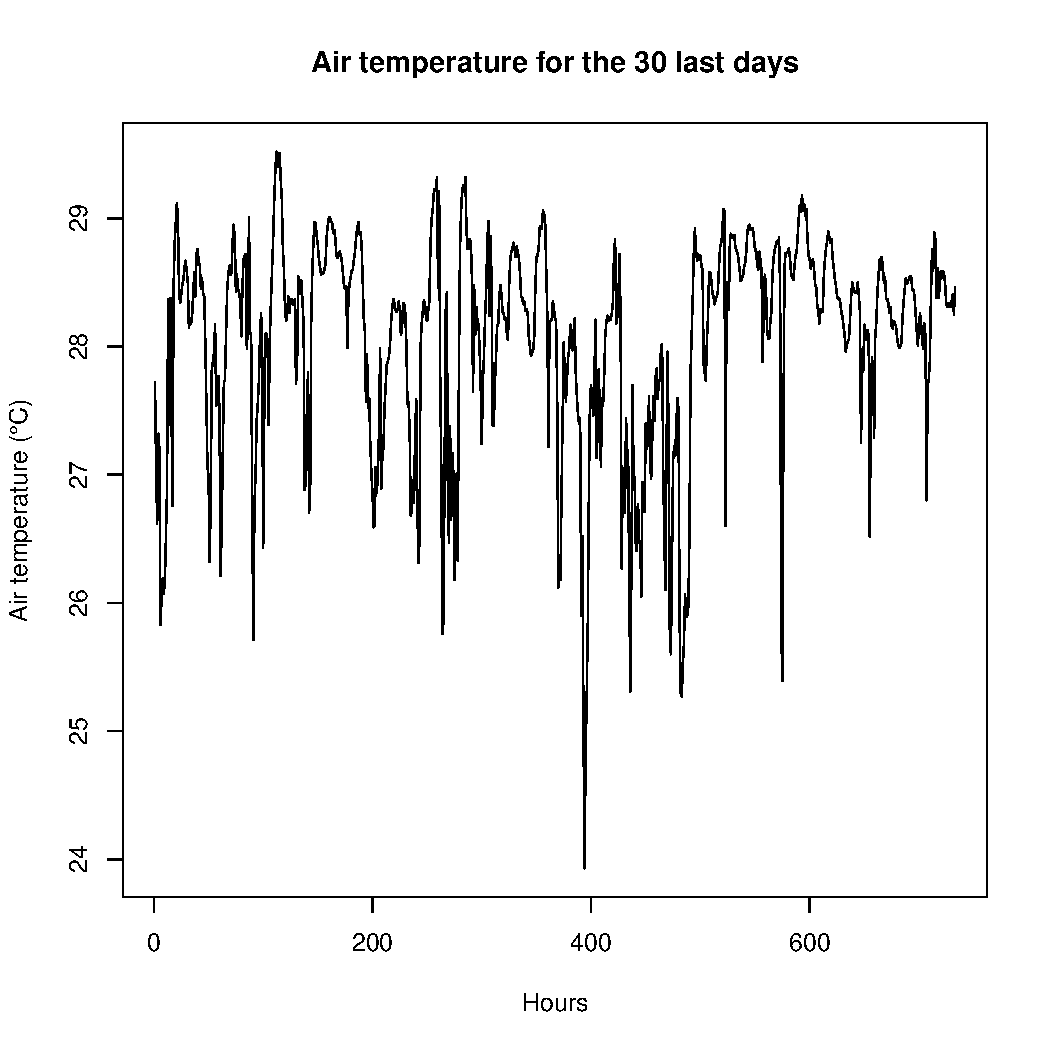
\includegraphics[width=0.6\linewidth]{Air2.pdf}
        \caption{Plot of the temperature the last 30 days}
        \label{air2}
    \end{center}
\end{figure}
\begin{figure}
    \begin{center}
        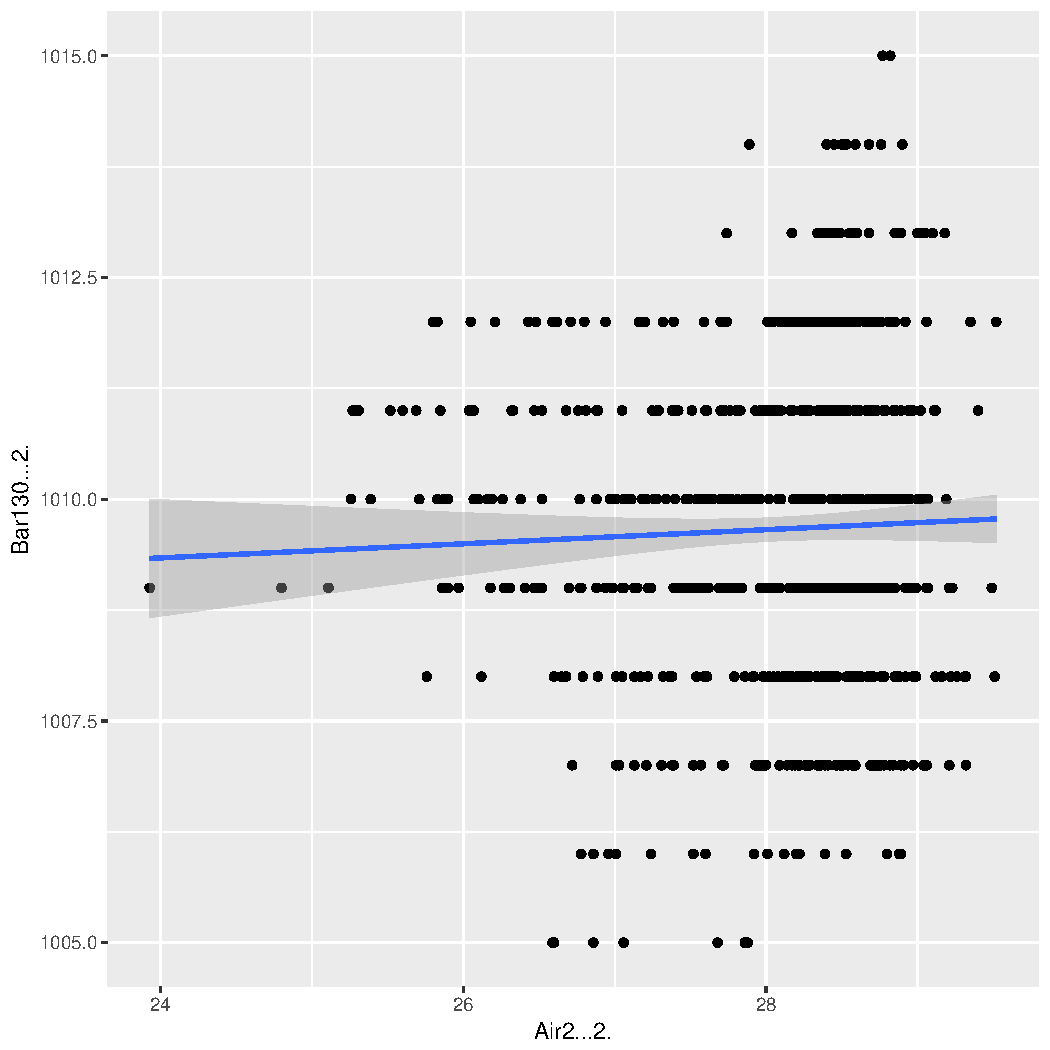
\includegraphics[width=0.6\linewidth]{PresTemp.pdf}
        \caption{Plot of the data of the first barometerfor against the air temperature for the last 30 days}
        \label{prestemp}
    \end{center}
\end{figure}

We use the correlation function of R to see if a correlation exists. We obtain a correlation coefficient of $0.0.04$ wich is far from 1, and a p-value of $0.3259$. Thus, we cannot conclude that there is a significant correlation between the two barometers.

\subsection*{Question 5}
Using the built-in lm R function, we find a equation of the linear model such as $y = 7.958e-02x + 1.007e+03$. We then use the summary function on the linear model, and see that the signification level is $0.3259$. Thus, we cannot say that our linear model is relevant.

\subsection*{Question 6}
Even though the two data are different on the physical approach, I think it could make sense to test if they have the same distribution. Indeed, the statistical distribution of the values it takes are not influenced by the physical nature of these parameters which could follow any distribution. It could then be interresting to do a one sample Kolmogorov-Smirnov test. Though, I don't see any point to compare one varaible to the other with the same test.

\end{document}
